%%% 1 Introduction/ %%%
\chapter{Introduction}\label{ch:intro}
%WHAT - what the reader needs to know to understand the presented 
%work, explain the background of research
Any online platform where users communicate with each other for different
purposes (e.g., digital transaction, news or file sharing) can be termed as an
online interaction system. Statistics~\cite{InternetWorldStat} suggest that
there are approximately 4 billion internet users worldwide and this number is
only increasing with each passing day. Internet live
stats~\cite{InternetLiveStat} is an online service that provides live
statistics on various online activities such as blog posts, social media usage,
internet traffic and emails sent.  Given the diversity of internet users, one
can reasonably assume that not all online interactions happen between known
entities. Depending on the nature of this interaction, the result can have a
significant impact on interacting entities. For instance, the failure of an
interaction that involves buying a house is not the same as failing to receive
a high-quality music file. To prevent severe damage that might result from a
failed transaction, trust frameworks and reputation model of the interaction
system plays a crucial role. They attempt to prevent harm by giving enough
information to predict the outcome.
%and therefore can be stated as a soft
%security mechanism. Rasmusson, Lars and Jansson,
%Sverker~\cite{rasmusson1996simulated} first used this term to describe the idea
%of identifying malicious users and preventing harm to other users in the
%context of secure open electronic commerce. Here, it is up to the individuals
%rather than the software to maintain security.
\begin{wrapfigure}{l}{0.6\textwidth}
	\begin{center}
		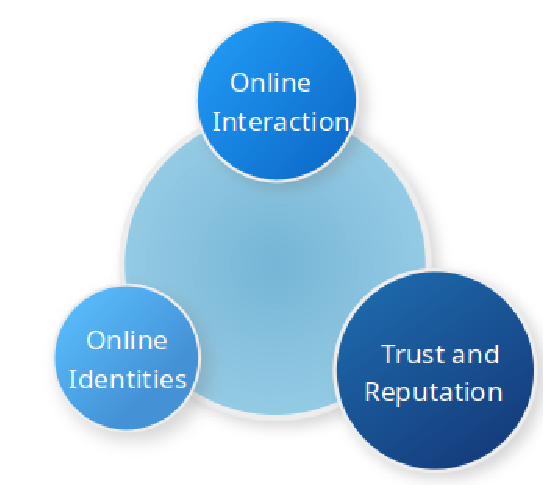
\includegraphics[width=0.5\textwidth]{Images/Introduction.eps}
		\caption{Online identities and their interaction}}
		\label{fig:introduction}
	\end{center}
\end{wrapfigure}
The risk of failure or probability of success when transacting with an entity
is reliant on the information provided by the underlying reputation system.
This information is usually presented in the form of trust scores assigned to
each online identities. Before engaging in an online transaction, the entities
need to select the online identity of the user with whom they intend to
interact. The interaction can then take place whose outcome is observed and
stored by the reputation system to update the current trust value further. As
can be seen in figure~\ref{fig:introduction}, the collection of online
identities, their interaction and inference of trust scores is a continuous
process. Examples of reputation systems in use by current online interaction
platform are eBay~\footnote{https://www.ebay.com/}, which is an e-commerce
platform, stackExchange~\footnote{https://stackexchange.com/}, which is a Q \&
A platform and Reddit~\footnote{https://www.reddit.com/}, which is a content
rating and discussion platform. The trust score of users is based on their
feedback, positive/negative ratings, upvotes/downvotes from the participants
with an equal privilege to interact with the system. The final score aggregated
via these objective measures can either increase or lower the reputation of the
user and limit their interaction ability. A general trust framework and a good
reputation model to specify the rules of interaction between online identities
and the extraction of useful information from them is, therefore, essential to
maintaining the security of an online interaction system. Equally significant
is to protect the integrity of this information such that they are reliable,
untampered (no deliberate alteration of data) and always available. Most of the
online interaction systems make use of a client-server architecture to serve
and govern the data usage. As such, the system is centralized and prone to both
external attack and internal modifications. If the server node fails, then the
whole network fails since none of the clients can access the data anymore. 
\begin{figure}
	\begin{center}
		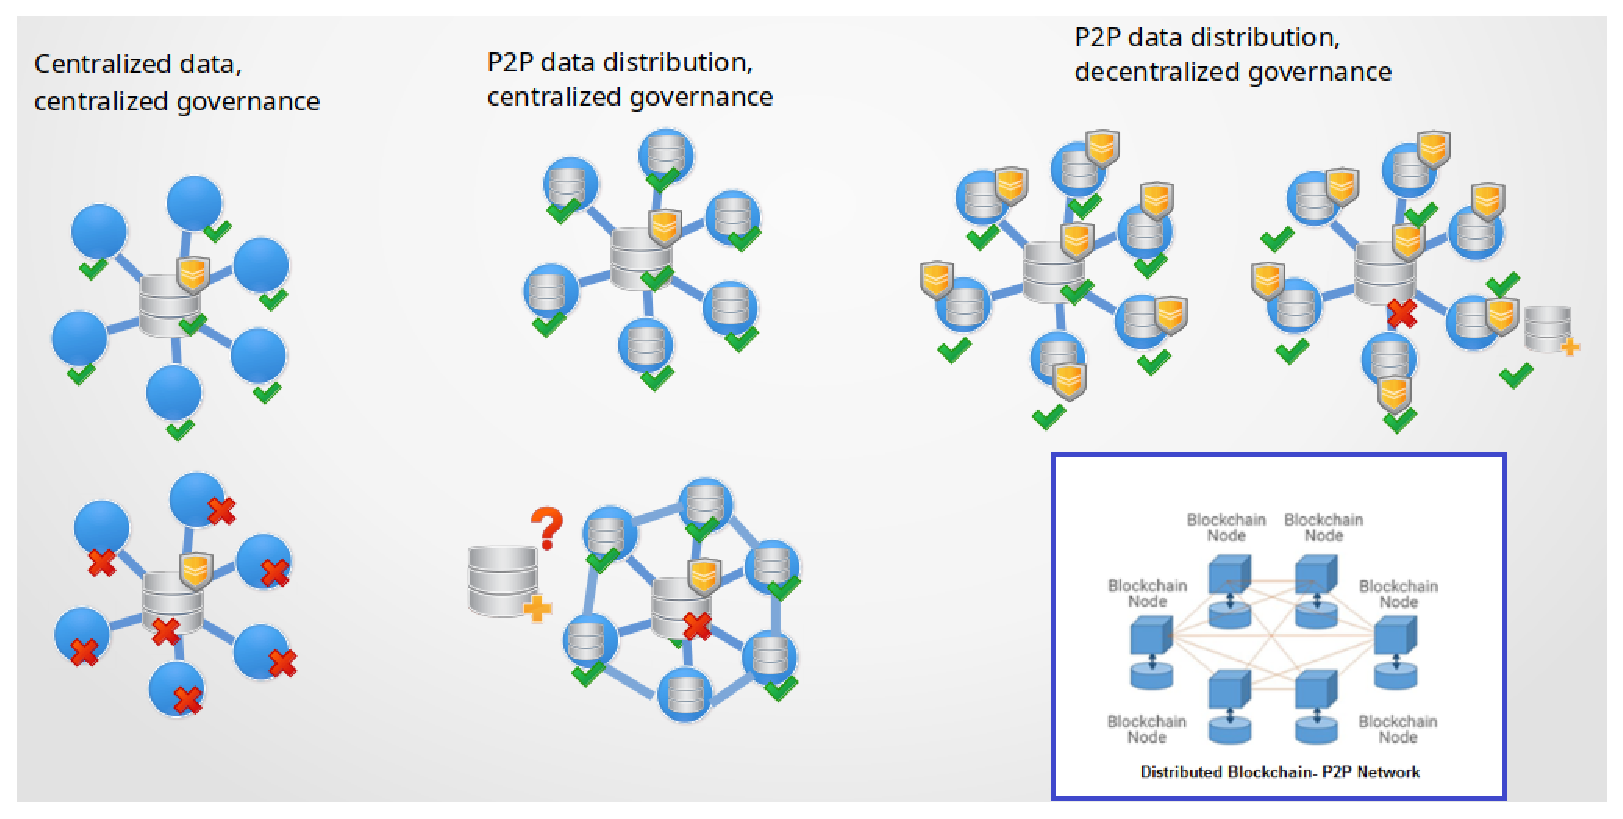
\includegraphics[width=1.0\textwidth]{Images/WhyBlockchain.eps}
		\caption{Centralized Vs. decentralized network}
		\label{fig:WhyBlockchain}
	\end{center}
\end{figure}
An alternative architecture that is primarily utilized by file sharing systems
is a Peer-to-Peer (P2P) network, and reputation-based trust management system
for them exists as well~\cite{selcuk2004reputation}. In a P2P network, all
nodes (peers) can act as both client and server, i.e., a peer can both request
and serve data. Thus, if one node fails then, clients can still request data
from other nodes in the network. This architecture solves the problem by P2P
data distribution. However, the governance of data is still centralized such
that clients still need to wait for a particular node that has the privilege to
add new data. This leaves the possibility for an online service running on
these networks to be shut down by a central authority.  Examples include the
shutdown of P2P services such as Megaupload~\cite{kang2012megaupload}  and
Napster~\cite{stern2000napster}. Therefore, this system is still vulnerable to
internal modifications as it is reliant on a trusted entity (administrator
node). Blockchain~\cite{atzori2015blockchain} solves these issues by providing
P2P data distribution along with decentralized governance.
Figure~\ref{fig:WhyBlockchain} shows the difference between the models
mentioned above. \\
\begin{figure}
	\begin{center}
		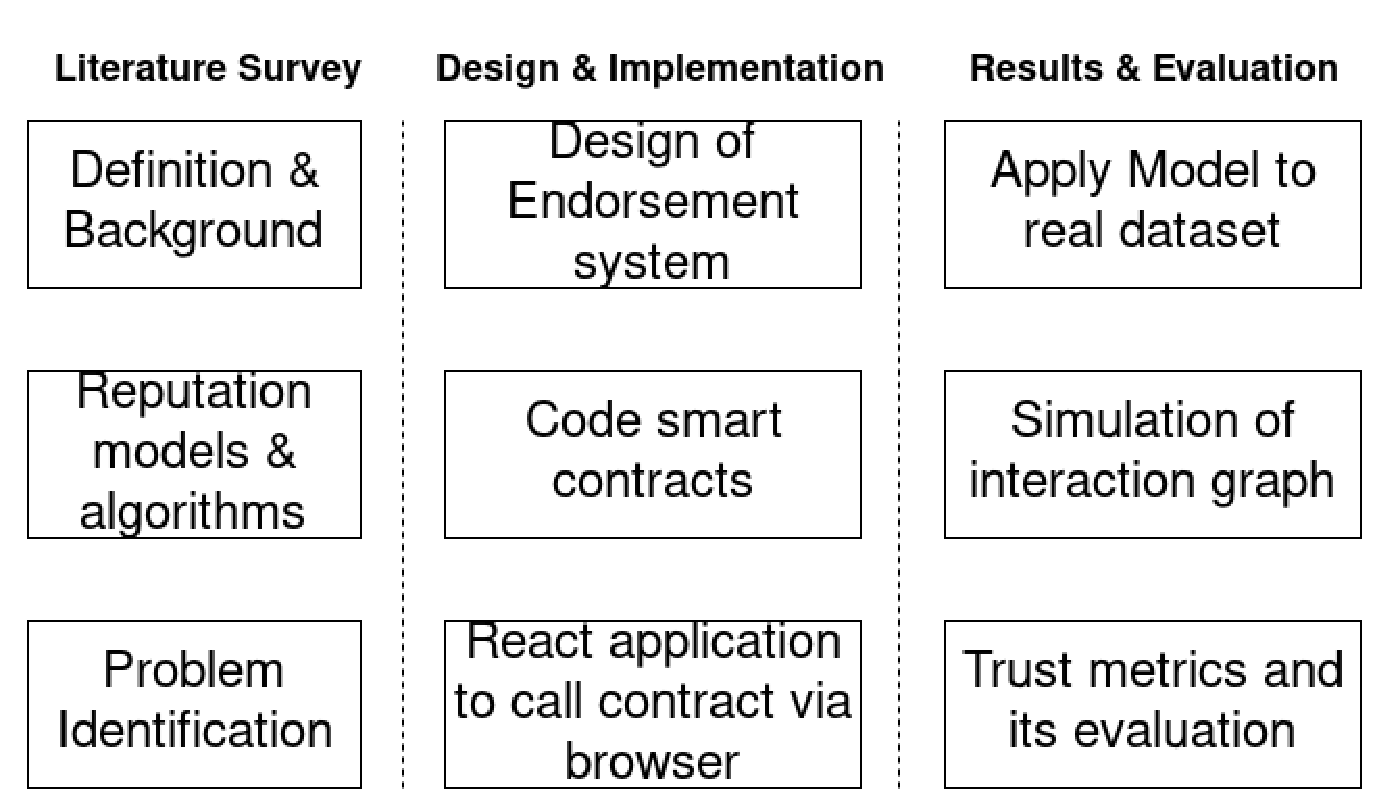
\includegraphics[width=0.9\textwidth]{Images/workflow.eps}
		\caption{Workflow of the project}
		\label{fig:thesisSteps}
	\end{center}
\end{figure}
This master's thesis project, therefore, proposes the use of blockchain
technology and smart contracts to model a trust framework and implement a
reputation system. The initial step of the project was the identification of
relevant concepts by performing a literature survey on existing reputation
models, properties of graph-based algorithms and its relevance to the project.
The survey motivated the design of a solution, wherein the proposed model,
participating entities can endorse each other.  Based on assumptions about
different possibilities of endorsement behavior that may occur, trust metrics
were defined in a way that honest participation would be encouraged. The
definition of honest and malicious participation from the perspective of an
endorsement network is discussed. A method to collect and quantify this
endorsement information to assign a trust score to each entity is presented. To
assess the working of the proposed model, it is applied to an existing real
dataset. Computation of trust scores for each participant based on the defined
trust metrics is presented. The simulated graph and computed trust scores do
support the defined metrics. A discussion of relevant threat models on
reputation systems and how the proposed model addresses them is performed.
Figure~\ref{fig:thesisSteps} gives the workflow of this master's thesis
project.
\section{Definition}
This section aims to define trust and reputation as it exists and discuss the
classification of its measure. Similarly, a brief overview of blockchain
technology and its definition is presented. 

%Trust and reputation can have different meanings based on context. Similarly,
%blockchain still lacks a standard definition. As such, this section aims to
%provide a general introduction and definition that will be followed by this
%master's thesis project. 

\subsection{Trust and Reputation}
Trust encompasses a broad spectrum of domains and is context dependent.
Therefore, its definition varies based on context and discipline and as such
lacks collective consensus among researchers~\cite{mcknight1996meanings}.
Using the classification from McKnight et al., 1996~\cite{mcknight2001trust},
trust can be either Personal/Interpersonal, Dispositional or
Impersonal/Structural.  Personal trust is when one person trusts another
specific person, persons, or things in a particular situation. Interpersonal
trust involves more than one trusting entities. i.e., two or more people (or
groups) trust each other.  Dispositional trust refers to a more general trust
that is based on the personality attribute of the trusting party. i.e., an
entity is more likely to trust other entity based on their attitude and is
cross-contextual. While the trust mentioned above are implicitly directed
towards a person, impersonal/structural trust refers to the trust in
institutional structure.  i.e., it is based on belief in regulatory enforcement
such as by contract law, judiciary systems rather than belief in involved
parties.\\

Trust can be generally seen as an entity's reliance on another interacting
entity to perform a specific set of the task given a specific situation.  As
pointed out by Gambetta et al.~\cite{gambetta2000can} ``Trust is the subjective
probability by which an agent assesses that other agent or group of agents will
perform a particular action that is beneficial or at least not detrimental.
"For an entity, $'A'$ to trust another entity ${'B'}$ or to evaluate $B's$
trustworthiness, the reputation of ${'B'}$ plays a central role. Broadly
defined, \textit{reputation} is the perception of an individuals character or standing.
Like trust, reputation is context-dependent. e.g., Alice may be trusted to
answer linux questions efficiently but not windows related
questions~\cite{zacharia2000collaborative}. A significant difference between
trust and reputation is that the former takes the subjective measure as input
whereas the latter takes an objective standard (e.g., transaction history,
ratings) as an input to yield a resulting score that can aid in detecting
reliability/trustworthiness of an
entity~\cite{Sabater2005,castelfranchi2000trust}. \\

Previous survey~\cite{ josang2007survey} has classified trust and reputation
measures as either subjective or objective measure. This classification is
further divided into specific or general. A subjective measure is based on an
individual's perspective and has no formal metrics.  Specific, subjective
measures imply a subjective perception of an entity for a specific ability,
such as package delivery time of a seller or average response time. One way of
measuring this is via survey questionnaires that ask specific questions. On the
other hand, a general, subjective measure, aggregates all the individual scores
and provides an average standing of the user on the network.  e.g., the
difference between positive and negative ratings used by eBay to give an
average rating.\\
An objective measure is used for product tests that can have some formal
criteria on which to rely on. e.g., hard disks can be measured based on
performance metrics such as transfer rate, access time, CPU usage. A specific,
objective measure takes an objective measure for a specific metric. i.e., how
good is a transfer rate for a particular hard disk Whereas, a general,
objective measure accounts for all the relevant aspects and averages the
performance to give an average rating/score on a specific scale. \\

The table below shows the classification of trust and reputation measures as
discussed above based on~\cite{ josang2007survey}: 
%The classification of trust and reputation measures based on previous survey   
 \begin{center}\label{table:classificationTrust}
	\begin{tabularx}{\textwidth }{|X| X| X| }
		\hline
		 & Specific, vector-based & General, Synthesized \\
		 \hline
		Subjective & Survey questionnaires & eBay, voting \\
		\hline
		Objective & Product tests & Synthesised general score from product tests \\
		\hline
		\caption{Classification of trust and reputation measures.}
	\end{tabularx}
\end{center}
Individuals in online systems are identified by their online identities which
can be anything and not necessarily linked to their real-world identities.
Online identities play a crucial role in digital interaction and require
unknown entities to trust each other based on the reputation system of the
platform in use. Trust and reputation can be seen as a soft security mechanism
where it is up to the participants rather than the software/system to maintain
security. By definition, a security mechanism~\cite{stallings2017cryptography}
is a process (or a device incorporating such a process) that is designed to
detect, prevent, or recover from a security attack. Unlike hard security
mechanism such as access control, capabilities, authentication where a user can
be allowed or rejected access to the resource, reputation system do not provide
a method to block or detect a security attack directly. However, they define a
process to identify malicious users and avoid them from harming other users in
the system. Rasmusson, Lars and Jansson, Sverker~\cite{rasmusson1996simulated}
first used this term, to describe the idea of identifying malicious users and
preventing harm to other users in the context of secure open electronic
commerce. Reputation system needs to continuously receive feedback about the
user's behavior and maintain an updated record of users. It provides a way to
calculate the probability of success or risk of failure of a transaction
between interacting parties. 

%gather statistics on attacks, fraud data. 
%the trust value obtained in the endorsement network can be integrated with 
%existing reputation model of other transaction network and both combined 
%should give a higher accuracy for trustworthiness measure of entities(assumption)

\subsection{Blockchain}
Blockchain can be defined as a distributed record of state changes that let
anybody on the network audit state changes and prove with mathematical
certainty that the transactions transpired according to the blockchain
protocol. There exist several definitions of blockchain technology each
specific to their closest use case. A formal standard definition of Blockchain
is under development as ISO/TC 307~\cite{ISOTC307}.\\
Vitalik Buterin, the founder of Ethereum, defines it this
way~\cite{VitalikVisions}: "A blockchain is a magic computer that anyone can
upload programs to and leave the programs to self-execute, where the current
and all previous states of every program are always publicly visible, and which
carries a very strong cryptoeconomically secured guarantee that programs
running on the chain will continue to execute in exactly the way that the
blockchain protocol specifies."\\
%\begin{quote}
%	\centering
%	"A blockchain is a magic computer that anyone can upload programs to and
%	leave the programs to self-execute, where the current and all previous
%	states of every program are always publicly visible, and which carries a
%	very strong cryptoeconomically secured guarantee that programs running on
%	the chain will continue to execute in exactly the way that the blockchain
%	protocol specifies."
%	\footnote{\url{https://blog.ethereum.org/2015/04/13/visions-part-1-the-value-of-blockchain-technology}} 
%\end{quote}
This definition provides a broad overview of what blockchain does. As a
continually developing discipline, it keeps adapting to a new definition while
maintaining the essence. The major innovation of blockchain as an architecture
is distributed, decentralized trustless (i.e., verification of transaction
doesn't require a trusted third party or require transacting parties to trust
each other) transactions~\cite{Bitcoin_Satoshi}. It completely removed the need
for an intermediary trusted third party by building trust in the system itself.
One dimension of trust as mentioned by ~\cite{miller2010trust} is trust in data
which is based on integrity of stored data.  Trusting data ensures that the
data is appropriate for use: accurate, precise, available, and
uncorrupted~\cite{miller2010trust}.  Blockchain achieves this by use of
cryptographic schemes mentioned in section~\ref{sec:cryptography}.
%assuring
%tamper-resistant, fault-tolerance, zero-downtime
%characteristics~\cite{swan2015blockchain}. 
\newpage

% ~\cite{enoughBitcoinForEthereum}
 
\section{Motivation}
%WHY: why is it interesting to study reputation system/trust 
% why blockchain based solution is relevant/interesting
Consider a simple scenario where Alice wants to buy a pair of headphones for
which she browses a ``buy/sell'' platform. When she finds a relevant product on the
platform published by Bob, unknown entity to Alice, the success or failure of
the transaction is dependent on two factors that may or may not be transparent.
\paragraph{Bob's reputation:} Bob's reputation can be inferred from his history
of transactions, ratings provided by previous buyers that have dealt with him,
reputation system of the platform in use, the integrity of all these relevant
data.  
\paragraph{Platform's reputation:} Reputation of the platform can also be
inferred similarly based on the history of services it has been able to
provide, a general perception in the community, etc.  Here, the platform in use
acts as the trusted third party that Alice must trust to present correctly
computed, untampered data about Bob. The entity claiming to be Bob could be
Eve, who found a way to bypass the platform's security and inflate his
reputation.  Eve could delete the ad and associated account when the payment is
complete, or she could gather Alice's details to misuse it later.  Any
malformed decision on the trustworthiness of an entity could be expensive and
deal severe damage to the user. \\
Statistics suggest that online shopping is the most adapted online
activity~\cite{experian}. Reports by Experia~\cite{experian} and
Javelin~\cite{javelin} indicate that E-commerce fraud has risen to
30\% in 2017 from 2016 while identity fraud victims have risen by 8\% in 2017
(16.7 million U.S victims). 
%Additionally, reports on fake news
%\footnote{\url{https://journalistsresource.org/studies/society/internet/fake-news-conspiracy-theories-journalism-research}}$^{,}$\footnote{\url{https://www.prnewswire.com/news-releases/84-percent-of-businesses-could-reduce-fraud-risk-if-certain-about-customers-identity-300587192.html}}
%that leads to spread of misinformation from malicious users or portals, attack
%on an existing system continues.
A recent report of data breach on Finnish Enterprise Agency for
Helsinki~\cite{finland}~\footnote{https://liiketoimintasuunnitelma.com/}
exposed 130,000 users login details.
%while Facebook has admitted to the compromise of
%2.2 billion of its user's data
%\footnote{\url{https://thenextweb.com/facebook/2018/04/05/zuckerberg-facebooks-2-billion-users-assume-data-compromised/}}.
%\footnote{\url{https://thehackernews.com/2018/04/facebook-data-privacy.html}}.
While there are several security reasons that have led to attack at such scale.
One major reason is the client-server architecture where everything is stored
on a centralized server and data flows in and out from the same source. On the
other hand, distributing information over a decentralized network would require
a simultaneous attack to achieve the same effect, thereby increasing the
difficulty level of attack. Similarly, Reputation models can help in measuring
the reliability of interacting entities so that users can make an informed
decision before participating in any transactions. Thus, a reputation system
should be secure, robust, always available and aim for higher accuracy. The use
of right reputation algorithms with Blockchain technology could help to ensure
trustworthiness of online entities with correctness of data and a high degree
of accuracy.  

%generalize a trust framework is, therefore, a riveting problem. Graph theory
%and network flow algorithms have been researched in both centralized and
%decentralized environment before. This thesis proposes a blockchain based
%solution to record users behavior and compute a trust score for each of them. 

\section{Purpose and research questions} \label{ResearchQuestions}
%Goal of thesis
%Research questions and approach that will be taken to answer 
%them in brief.
The primary goal of this master's thesis project is to use blockchain technology
and smart contracts to simulate an endorsement network where entities can
endorse each other based on physical or digital acquaintance. The endorsement
will be quantified to infer reputation score which in turn can yield a value
that can represent the impact the agent has made on the network.  The nodes and
their relationship will be studied to analyze honest or malicious
participation.  Generalization of this endorsement network to serve other use
cases shall be discussed as well. 

The research questions that this master's thesis project aims to address are : 
\begin{enumerate}
		\item How can graph theories and relevant reputation algorithms be used
			to model the interaction between entities and detect/identify
			honest and malicious nodes in the network? How can the interaction
			graph be modeled? \label{question1}
		\item What are the requirements for storing trust values and linking
			them to associated identities stored off a blockchain network? How
			can a blockchain application be built to define a general trust
			framework for a transactional network? How could the overall system
			architecture look like? \label{question2} 
		\item How can the discussed endorsement network ensure trustworthiness
			while also preserving users anonymity and how can it be generalized
			to other transactional network or added on top of it to serve other
			use cases such as content filtering, E-Commerce
			etc.?\label{question3} 
\end{enumerate}

\section{Scope} 
%Identify goal, objective, timeplan, deliverables, 
%what the project is supposed to do and the work required to meet 
%the objective
This master's thesis project attempts to answer all the research questions mentioned
in section~\ref{ResearchQuestions}. \\
\textbf{Research Question 1}\\
To answer research question 1, literature survey is performed on various
reputation algorithms and existing models. This survey follows with the
discussion on various analysis metrics and threat models that eventually leads to
graph simulation of endorsement network.  

\textbf{Research Question 2 } \\
Interpretation of nodes connections and quantification of scores for individual
nodes that represents trustworthiness based on score range is presented.
Comparative analysis of on chain vs. off-chain storage requirements is 
studied and analyzed. Overall system design and architecture is presented. 

\textbf{Research Question 3} \\
The endorsement network is analyzed against various network metrics to
show resilience to threat models. Discussion on other use cases and how the
endorsement model can be used on top of other systems is also presented.

%
%For research question\ref{question2}, interpretation and quantification of reputation
%scores and trust metrics will be manifested. Comparative analysis of on chain
%and off-chain storage requirements will be studied resulting in an overall
%design of endorsement system architecture. \\
%\textbf{Research Question 3}
%The endorsement network will be analysed against various network metrics to show resilience to threat models. Discussion on other use cases and how the endorsement model can be used on top of other system will be presented. 
%

%For research question\ref{question3}, relevant use cases will be presented, and the
%network will be tested on with various predefined cases and attack models to
%see how well it behaves in a dynamic environment. \\

\section{Structure of Report}
This paper is structured as follows. Chapter~\ref{ch:litrev} performs a
literature survey on the existing algorithms and their implementations.
Chapter~\ref{ch:background} provides a background overview of relevant concepts
necessary to understand the following sections. In chapter~\ref{ch:method},
system requirements and the approach taken for the model design is shown. It
shows the overall system design and architecture. Chapter~\ref{ch:results}
follows on with discussion of evaluation metrics and test methods and present
results representative of the designed model. Finally, conclusion and future
work is presented in chapter~\ref{ch:conclusion}. 
